
\documentclass[10pt,journal,cspaper,compsoc]{IEEEtran}
%
% If IEEEtran.cls has not been installed into the LaTeX system files,
% manually specify the path to it like:
% \documentclass[12pt,journal,compsoc]{../sty/IEEEtran}

\usepackage{fixltx2e}
% \usepackage{stfloats}
\usepackage{amsmath}
\usepackage{graphicx}
\usepackage{amsfonts}
\usepackage{amsthm}
%\usepackage{cite}
\usepackage{algorithm}
\usepackage{algorithmic}
\input{/Users/jovo/Research/latex/latex_commands.tex}
\hyphenation{op-tical net-works semi-conduc-tor}


\begin{document}

\title{Graph Classification using Signal Subgraphs}

\author{Joshua T.~Vogelstein,
		William~R.~Gray,
        R.~Jacob~Vogelstein,
        and~Carey~E.~Priebe% <-this % stops a space
\IEEEcompsocitemizethanks{\IEEEcompsocthanksitem J.T. Vogelstein and C.E. Priebe are with the Department
of Applied Mathematics and Statistics, Johns Hopkins University, Baltimore, MD 21218.\protect\\
% note need leading \protect in front of \\ to get a newline within \thanks as
% \\ is fragile and will error, could use \hfil\break instead.
E-mail: joshuav@jhu.edu
\IEEEcompsocthanksitem W.R. Gray and R.J. Vogelstein are with the Johns Hopkins University Applied Physics Laboratory, Laurel, MD, 20723.}% <-this % stops a space
\thanks{}}

% The paper headers
\markboth{IN PREP}%
{Graph Classification}

\IEEEcompsoctitleabstractindextext{%
\begin{abstract}
%\boldmath
The abstract goes here.The abstract goes here.The abstract goes here.The abstract goes here.The abstract goes here.The abstract goes here.The abstract goes here.The abstract goes here.The abstract goes here.The abstract goes here.The abstract goes here.

The abstract goes here.The abstract goes here.The abstract goes here.The abstract goes here.The abstract goes here.The abstract goes here.The abstract goes here.The abstract goes here.The abstract goes here.The abstract goes here.The abstract goes here.The abstract goes here.The abstract goes here.The abstract goes here.
\end{abstract}

% Note that keywords are not normally used for peer review papers.
\begin{keywords}
Computer Society, IEEEtran, journal, \LaTeX, paper, template.
\end{keywords}}


% make the title area
\maketitle
\IEEEdisplaynotcompsoctitleabstractindextext
\IEEEpeerreviewmaketitle



\section{Introduction}

\IEEEPARstart{G}{raphs} are becoming increasingly popular vehicles for data representation, spanning fields from optical character recognition \cite{}, to chemistry \cite{}, to neuroscience \cite{}.  While statistical inference techniques for vector-valued data are widespread, statistical tools for the analysis of graph-valued data are relatively rare \cite{}. In this work we propose and analyze a relatively simple yet rich random graph model---sufficiently simple to characterize its asymptotic properties, and sufficiently rich to afford useful empirical applications.  For concreteness, we consider the task of \emph{graph classification}: given a collection of graphs and their corresponding classes, can we accurately estimate the class of a new graph lacking a class label?  Our approach is statistical in nature. We first define a graph/class model.  This model admits that the class-conditional signal is encoded in a subset of edges, the \emph{signal subgraph}. Finding the signal subgraph amounts to providing an understanding of what are the differences between the two classes of graphs.  This approach is quite different from quantifying a number of graph invariants (such as clustering coefficient), and building a classifier in a graph invariant space.  Specifically, in the proposed model-based approach, we use both (i) the vertex labels and (ii) graph structure to help classify.  To our knowledge, this is the first proposed strategy using both of those cues.  We demonstrate via proofs, simulation, and a neurobiological data set (MR connectomes \cite{}) that ignoring one or the other of these cues significantly degrades one's ability to classify.

\section{Methods} % (fold)
\label{sec:methods}

% section methods (end)

\subsection{Setting}

Let $\GG: \Omega \mapsto \mc{G}$ be a graph-valued random variable with samples $G_i$.  Each graph is defined by a set of $V$ vertices, $\mc{V}=\{v_i\}_{i \in [V]}$, where $[V]=\{1,\ldots, V\}$, and a set of edges between pairs of vertices $\mc{E}$, where $|\mc{E}| \leq V^2$. An adjacency matrix, $A$, is a binary $V \times V$ matrix listing  which vertices share an edge. Let $Y:\Omega \mapsto \mc{Y}$ be a discrete-valued random variable with samples $y_i$.  Assume the existence of a collection of $n$ exchangeable samples of graphs and their corresponding classes from some true but unknown joint distribution: $\{(\GG_i,Y_i)\}_{i \in [n]} \overset{exch.}{\sim} F_{\GG,Y}$. Our aim (or exploitation task) is then to build a graph classifier that could take a new graph, $g$, and correctly estimate its class, $y$, assuming that they are jointly sampled from the same distribution, $F_{\GG,Y}$.  Moreover, we are interested solely in graph classifiers that are \emph{interpretable} with respect to the vertices and edges of the graph. In other words, manifold learning, feature extraction, and related approaches are inadmissible.  

\subsection{Model} % (fold)
\label{sub:model}

A model defines the set of admissible distributions.  In the graph classification domain, we consider the model, $\mc{F}_{\GG,Y}$, which includes all joint distributions over graphs and classes under consideration: $\mc{F}_{\GG,Y}=\{F_{\GG, Y} : \bth \in \bTh\}$, where $\bth$ indexes each distribution, and must live in $\bTh$.  Two ``standard'' approaches for tackling a classification problem are (i) the \emph{generative} approach and (ii) the \emph{discriminative} approach.  In a generative strategy, one deconstructs the joint distribution into a product of a likelihood term and a prior term:  $F_{\GG,Y}=F_{\GG | Y}F_Y$.  In a discriminative strategy, one deconstructs the joint distribution into a posterior term and a marginal term: $F_{\GG,Y}=F_{Y | \GG}F_{\GG}$.  We proceed using a hybrid generative-discriminative approach whereby we describe a generative model and place constraints on the discriminant boundary.

First,  assume that each graph has the same set of labeled vertices, so that all the variability in the graphs is in the adjacency matrix, which implies that $F_{\GG,Y}=F_{A,Y}$. Second, assume edges are independent, that is: $F_{A,Y}=\prod_{u,v \in \mc{E}} F_{A_{uv},Y}$.  Now, consider the generative deconstruction, and let $F[A_{uv} | Y=y]=f_{uv|y}$ and $F_Y=\pi_Y$,  noting that $F_{\GG,Y}=f_Y \pi_Y$.  Third, assume the existence of a class-conditional difference, that is $f_{uv|0} \neq f_{uv|1}$ for some $(u,v) \in \mc{E}$, and denote the edges satisfying that condition comprise the \emph{signal subgraph}, $\mc{S}=\{(u,v) \in \mc{E}: f_{uv|0} \neq f_{uv|1}\}$.  Fourth, for concreteness, assume that the graphs are \emph{simple} graphs, that is, undirected, with binary edges, and lacking (self-) loops.  Thus, the likelihood of an edge between vertex $u$ and $v$ is given by a Bernoulli random variable with a scalar probability parameter:  $f_{uv|y}=\text{Bern}(A_{uv}; p_{uv|y})$. Together, these four assumptions imply the following model: 
\begin{align}
\mc{F}_{\GG,Y}=\{F_{\GG, Y}=\prod_{uv \in \mc{S}} \text{Bern}(A_{uv|Y}; p_{uv|Y}) \pi_Y :  \bth \in \bTh\},
\end{align}
where $\theta$ is composed of three parameters: $\mc{S}$, $\mb{p}$, and $\mb{\pi}$, each of which lives in a parameter space.  First, the signal subgraph parameter, $\mc{S}$, must be a non-empty subset of all possible edges: $\mc{S} \subseteq \mc{E} \cap \mc{S} \neq \emptyset$.   Second, the likelihood term parameter, $\mb{p}=\{p_{uv|y}\}_{uv \in \mc{S}, y \in \mc{Y}}$, is constrained in that each term must be between zero and one: $p_{uv|y} \in (0,1)$.  Third, the prior terms, $\mb{\pi}=\{\pi_y\}$, must be greater than zero and sum to one: $\pi_y \geq 0, \sum_y \pi_y=1$.  Thus, given a specification of the signal subgraph, the class-conditional likelihood of an edge in each the signal subgraph, and class-priors, one completely defines a possible joint distribution over graphs and classes.


% subsection model (end)

\subsection{Classifier} % (fold)
\label{sub:classifier}



Formally, we say that a graph classifier, $h$, is any function satisfying $h: \mc{G} \mapsto \mc{Y}$.  We desire to obtain the best possible classifier, $h_*$. To determine which is best, we first define a loss function, which rates the performance of each classifier as a function of the distribution: $\ell: \mc{F} \times \mc{H} \mapsto \Real_+$, where $\mc{H}$ is the space of admissible classifiers.  We choose to measure classification performance by the expected misclassification rate:
\begin{multline}
\ell_F(h) = \EE_{F}[h(G) \neq Y] =\\ \int
% _{g \in \mc{G}, y\in \mc{Y}} 
F[h(g) \neq y] F[g,y] dgdy.
\end{multline}
The best classifier (under model $\mc{F}$ and loss-function $\ell$) is the classifier with minimal loss: $h_*=\argmin_{h \in \mc{H}} \ell_F(h)$.  Such a classifier is called \emph{Bayes optimal}, and the error associated with such a classifier is called \emph{Bayes error} or \emph{Bayes risk}.  It can be shown that the classifier that maximizes the class-conditional posterior, $F_{Y | \GG}$ is Bayes optimal [1]:
\begin{align} \label{eq:map}
h_*(g) &= \argmin_{h \in \mc{H}} \ell_F(h) = \argmax_{y \in \mc{Y}} F[y|g] 
\nonumber \\ &= \argmax_{y \in \mc{Y}} F[g|y] F[y].
\end{align}
Given the proposed model, Eq. \eqref{eq:map} can be further factorized using the above four assumptions:
\begin{align}
\argmax_{y \in \mc{Y}} F[g|y] F[y] 
% &= \argmax_{y \in \mc{Y}} F[a|y] F[y] 
% \nonumber \\ &= \argmax_{y \in \mc{Y}} \prod_{u,v \in \mc{E}} f_{uv | y} \pi_y 
% \nonumber \\ &= \argmax_{y \in \mc{Y}} \prod_{u,v \in \mc{S}} f_{uv | y} \pi_y 
% \nonumber \\ 
&= \argmax_{y \in \mc{Y}} \prod_{u,v \in \mc{S}} \text{Bern}(a_{uv}; p_{uv|y}) \pi_y.
\end{align}
Unfortunately Bayes optimal classifiers are typically unavailable. In such settings, it is therefore desirable to construct a classifier estimate from a set of \emph{training data}. Formally, let $\mc{D}_n$ denote the data corpus, assumed to be sampled exchangeably from the true but unknown distribution: $\mc{D}_n=\{(\GG_i,Y_i)\}_{i \in [n]} \overset{exch.}{\sim} F_{\GG, Y}$.  Given such a training corpus, and a new, as yet unclassified graph, $g$, an estimated classifier predicts the true (but unknown) class of $g$ by utilizing the training corpus: $\mh{h}_n: \mc{G} \times (\mc{G} \times \mc{Y})^n \mapsto \mc{Y}$.  When a model, $\mc{F}_{\GG,Y}$ is specified, a beloved approach is to use  a  \emph{Bayes plug-in classifier}. Due to the above simplifying assumptions, the Bayes plug-in classifier for this model is defined as follows.  First, estimate the three model parameters (1) $\mc{S}$, (2) $\mb{p}=\{p_{uv|y}\}_{uv \in \mhc{S}, y \in \mc{Y}}$, and (3)  $\mb{\pi}=\{\pi_y\}$. Second, plug those estimates into the above equation.  The result is a Bayes plug-in graph classifier:
\begin{align}
\mh{h}_n(g) \defeq  \argmax_{y \in \mc{Y}} \prod_{u,v \in \mhc{S}}
\mh{p}_{uv|y}^{a_{uv}}(1-\mh{p}_{uv|y})^{(1-a_{uv})} \mh{\pi}_y,
\end{align}
where the Bernoulli probability is explicit. To implement such a classifier estimate, we require estimators for estimating the above three estimands.

% subsection classifier (end)

\subsection{Estimators} % (fold)
\label{sub:estimators}


In this section we describe algorithms to estimate the parameters of our model.  An \emph{estimator} is a function that maps samples from the sample space to the parameter space: $\bhth_n: \Xi^n \mapsto \bTh$; the output of this function is called the \emph{estimate}.  In the graph classification domain, for example, $\Xi=(\mc{G},\mc{Y})$.  In a slight abuse of notation, we will also refer to the sequence of estimators, $\bhth_1,\bhth_2, \ldots$, as an estimator.  We desire (a sequences of) estimators that satisfy the following five desiderata:

\begin{itemize}
	\item \textbf{Consistent}: an estimator is consistent if its sequence converges in the limit to the true value: $\lim_{n \conv \infty} \bhth_n = \bth$.  %When the parameter is multidimensional, an estimator can be consistent as the number of samples $n$ goes to infinity (i) but the dimensionality is fixed at $d$, or (ii) the dimensionality also goes to infinity.  The estimate resulting from using a consistent estimator is called \emph{asymptotically unbiased}.
	\item \textbf{Efficient}: an estimator is efficient if its sequence converges to the minimum variance: $\lim_{n\conv\infty} \text{Var}(\bhth_n) = \mc{I}_{\bth}^{-1}$.  %If one allows for infinite dimensional parameters, than it might be desirable to compute efficiency as both $n$ and $d$ approach infinity.  
	A maximally efficient estimator yields an estimate with \emph{minimum variance}.
	\item \textbf{Robust}: an estimator is robust if the resulting estimate is relatively insensitive to small model misspecifications.  Because the space of models is quite large (uncountably infinite), it is intractable to consider all misspecifications, so we only consider a few of them below. % Therefore, we consider robustness only to a small number of possible model misspecifications, as described in more detail below.
	\item \textbf{Quadratic complexity}: computational time complexity should be quadratic in the number of  or less.
	\item \textbf{Interpretable}: we desire that the parameters are interpretable with respect to a subset of vertices and/or edges.
\end{itemize}
In addition to the above categorical desiderata, we also desire ``nice'' finite sample and empirical performance.


\subsubsection{Signal Subgraph Estimators} % (fold)
\label{ssub:subsubsection_name1}


Na\"{i}vely, one might consider a search over all signal subgraphs, plugging each one in to the classifier, and select the best performing signal subgraph.  This strategy performs poorly with respect to at least two desiderata.  First, the number of signal subgraphs scales super-exponentially with the number of vertices (see Figure \ref{fig:numgraphs}, left panel). Specifically, the number of edges in a simple graph with $V$ vertices is $d_V=\binom{V}{2}$, so the number of unique subgraphs is $2^{\binom{V}{2}}$.  Searching over all of them is therefore ridiculously computationally taxing, and does not meet the quadratic complexity criteria. Second, the estimate will be determined partially by the chosen classifier.  This makes interpreting the results a bit tricky, as one cannot ascertain whether the signal subgraph chosen is the one that works best for the chosen classifier, or is the true signal subgraph (assuming that they could be different).  We therefore consider several alternatives.


% subsubsection subsubsection_name (end)



\begin{figure*}[tb!]
	\centering
		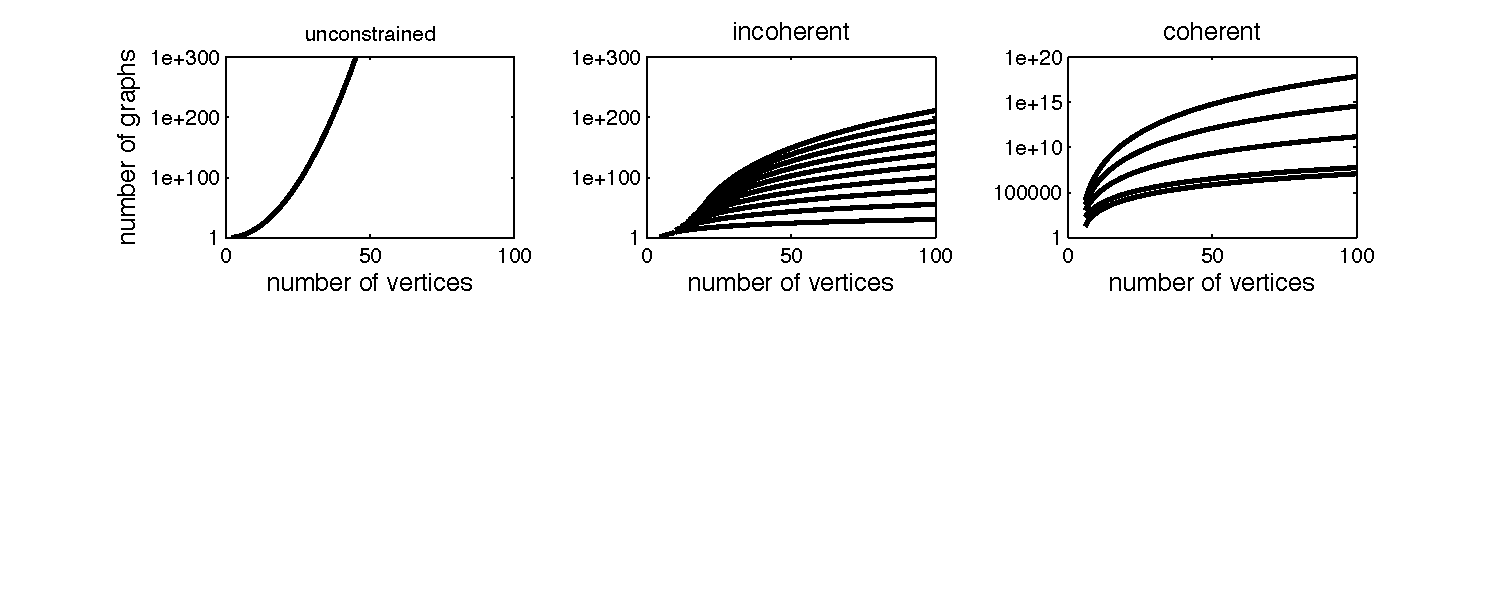
\includegraphics[width=1.0\linewidth]{../figs/num_of_graphs.pdf}
	\caption{Exhaustive searches for the signal subgraph, even given severe constraints, are computationally intractable for small graphs (e.g., with $\mc{O}(10)$ vertices).  Top panels show the number of unique simple subgraphs as a function of the number of vertices, $V$.  Note the ordinates are all log scale.   On the left is the unconstrained scenario, that is, all possible subgraphs for a given number of vertices.  In the middle panel, each line shows the number of subgraphs with fixed number of edges, $s$, ranging from 10 to 100, incrementing by 10 with each line.  The right panel shows the number of subgraphs for various fixed $s$ and only a single star-vertex, that is, all edges are incident to one vertex.  Bottom panels show a particular example subgraph via its adjacency matrix; white elements indicate an edge.}
	\label{fig:numgraphs}
\end{figure*}

\begin{figure*}[tb!]
	\centering
		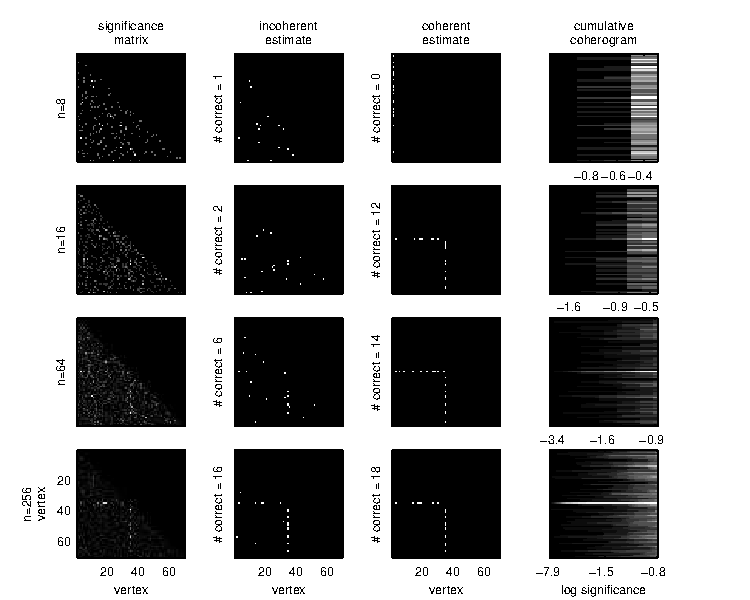
\includegraphics[width=1.0\linewidth]{../figs/homo_V70_s20_p10_q30_SigIncCohErogram.pdf}
	\caption{An example of the coherent signal subgraph estimate's improved accuracy over the incoherent signal subgraph estimate, for a particular homogeneous two-class model specified by: $\mc{M}_{70}(1,20;0.5,0.1,0.3)$. Each row shows the same columns but for increasing the number of graph/class samples.  The columns show the: (far left) negative log-significant matrix, computed using Fisher's exact test (lighter means more significant; each panel is scaled independent of the others because only relative significance matters here); (middle left) incoherent estimate of the signal subgraph; (middle right) coherent estimate of the signal subgraph; (far right) coherogram.  As the number of data samples increases (lower rows), both the incoherent and coherent estimates converge to the truth (the ordinate labels of the middle panels indicate the number of edges correctly identified).  For these examples, the coherent estimator tends to find more true edges.  The coherogram visually depicts the coherency of the signal; it is also converging to the truth---the signal subgraph here contains a single star-vertex.}
	\label{fig:4x4}
\end{figure*}



Before proceeding, recall that each edge is independent, which means that whether or not each edge is in the signal subgraph could be evaluated on its own.  Formally, consider a hypothesis test for each edge.  The null hypothesis is that the class-conditional edge distributions are the same, so $H_0: f_{uv|0}=f_{uv|1}$ for all $(u,v) \in \mc{S}$.  The composite alternative hypothesis is that they differ, $H_A: f_{uv|0} \neq f_{uv|1}$ for all $(u,v) \in \mc{S}$.  Given such hypothesis tests, one can construct test statistics using the data: $T=T_{uv}^{(n)}: \mc{D}_n \mapsto \Real_+$.  We reject the null in favor of the alternative whenever the value of the test-statistic is greater than some critical-value $c$: $T(\mc{D}_n)>c$.  We can therefore construct a \emph{significance matrix}: $\mb{T}_n=T_{uv}^{(n)}$, which encapsulates the significance of the difference for each edge between the classes.  

\paragraph{\emph{Incoherent Signal Subgraph Estimators}} % (fold)
\label{par:paragraph_name}


Assume the size of the signal subgraph, $|\mc{E}|=s$, is known.  The number of subgraphs with $s$ edges on $V$ vertices is given by $\binom{d_V}{s}$, where $d_V$ is the number of distinct edges in a graph with $V$ vertices; also super-exponential (see Figure \ref{fig:numgraphs}, middle panel). Thus searching them all is computationally intractable at this time.  When $s$ is given and the independent edge assumption is ``good'', one can choose the critical value \emph{a posteriori} to ensure that only $s$ edges are rejected, $c = \min_{c'} \II\{\sum_{(u,v) \in \mc{S}} \II \{T_{uv}^{(n)} > c'\}-s\}$,  where $\II\{\cdot\}$ is the identity function, equaling one whenever its argument is true, and zero otherwise.  Therefore, an estimate of the signal subgraph is the collection of $s$ edges with minimal test-statistics.  Formally, let $T_{(1)} < T_{(2)} < \cdots < T_{(d_V)}$ indicated the \emph{ordered} test statistics (dropping the superscript indicating the number of samplesfor brevity).  Then, the \emph{incoherent signal subgraph estimator} is given by: $\mhc{S}^{inc}_n$=$\{a_{(1)}, \ldots, a_{(s)}\}$, where $a_{(u)}$ indicates the $u^{th}$ edge ordered by significance of its test statistic, $T_{(u)}$.
% paragraph paragraph_name (end)

\paragraph{\emph{Coherent Signal Subgraph Estimators}}

In addition to the size of the signal subgraph, also assume that each of the edges in the signal subgraph are incident to one of $m$ special vertices called \emph{star vertices}. While this assumption further constrains the candidate sets of edges, the number of feasible sets still scales super exponentially (see Figure \ref{fig:numgraphs}, right panel).  Instead, we again take a greedy approach.  

First, compute the significance of each edge, as above, yielding ordered test-statistics, and rank edges by significance with respect to each vertex,  $E_{k,(1)} \leq E_{k,(2)} \leq \ldots \leq E_{k,(n-1)}$ for all $k \in \mc{V}$.  Second, recursively increase the critical value, $c$. With each iteration, assign each vertex a ``score'' equal to the number of edges per vertex with significance smaller than the critical value, $w_{(i);c}=\sum_{u \in [V]} \II\{T_{i,u} < c\}$.  If there exists $m$ vertices whose scores sum to greater than or equal the size of the signal subgraph, $s$, then stop iterating.  That is, find $\min_c !$ such that $\sum_{i} w_{(i);c}\geq s$.  Call the collection of $s$ most significant edges from within that subset the \emph{incoherent signal subgraph estimate}, $\mhc{S}^{coh}_n$.

\paragraph{\emph{Coherograms}}

In the process of estimating the incoherent signal subgraph, one builds a ``coherogram''.  Each row of the coherogram corresponds to a different critical value $c$, and each column corresponds to a different vertex $v$.  The $c,v$ element of the coherogram is the number of edges incident to vertex $v$ with significance smaller than $c$.  Thus, the coherogram gives a quick depiction of how coherent is the signal subgraph.


\subsubsection{Likelihood Estimators} % (fold)
\label{sub:likelihood}

The class-conditional likelihood parameters, $p_{uv|y}$, are relatively simple.  In particular, because the graphs are assumed to be simple, $p_{uv|y}$ is just an independent Bernoulli parameter for each edge in each class.  The maximum likelihood estimator (MLE), which simply the average value of each edge per class, seems to be a good choice:
\begin{align}
\mh{p}_{uv|y}^{MLE} = \frac{1}{n_y} \sum_{i | y_i = y} a_{uv}^{(i)},
\end{align}
where $\sum_{i | y_i=y}$ indicates the sum is over all data samples from class y. Unfortunately, the MLE has relatively poor finite sample properties.  In particular, if the data contains no examples of an edge in a particular class, then the MLE will be zero.  If the new to be classified graphs exhibits that edge, then the probability of it being from that class is zero, which we do not believe.  We therefore consider an estimator with better finite sample performance, the maximum a posteriori (MAP) estimator (other choices, such as an ML$_q$ estimator, might be better \cite{}).  The MAP estimator for a Bernoulli random variable requires specifying a prior.  Because the beta distribution is the conjugate prior to the Bernoulli distribution, it is a convenient choice: 
\begin{align}
F[ p_{uv|y} | \alpha, \beta] &= \text{Beta}(p_{uv|y}; \alpha,\beta)
\nonumber \\ &= \frac{1}{B(\alpha,\beta)}p_{uv|y}^{\alpha-1}(1-p_{uv|y})^{\beta-1}.
\end{align}
And because we have relatively little prior knowledge about the probabilities other than a disbelief with regard to zero, we choose a \emph{weakly informative prior} [cite], namely the uniform prior: $\alpha=\beta=1$. Given such a prior, the posterior distribution is simply: $\text{Beta}(\mt{\alpha}_{uv|y},\mt{\beta}_{uv|y})$, where $\mt{\alpha}_{uv|y}=\alpha+n_{uv|y}$, $\mt{\beta}_{uv|y}=\beta+(n_y-n_{uv|y})$, and $n_{uv|y}=\sum_{i | y_i = y} a_{uv}^{(i)}$.  The posterior is unimodal because both the parameters are greater than one [cite].  The mode (which is the maximum a posteriori estimate) is given by:
\begin{align}
\mh{p}_{uv|y}^{MAP} = \text{Beta}(\mt{\alpha}_{uv|y},\mt{\beta}_{uv|y}),
\end{align}
which we use for our likelihood estimates.
% subsection likelihood (end)



\subsubsection{Prior Estimators} % (fold)
\label{sub:prior_estimators}

The prior are the simplest.  The prior probabilities are Bernoulli, and we are only concerned with the case where $|\mc{Y}| \ll n$, so the maximum likelihood estimators are sufficient:
\begin{align}
\mh{\pi}_y = \frac{n_y}{n},
\end{align}
where $n_y=\sum_{i \in [n]} \II\{y_i = y\}$.

% subsection prior_estimators (end)


\subsection{Evaluation Criteria} % (fold)
\label{sub:evaluation_criteria}

The properties of the MAP and ML estimators for the likelihood and prior terms, respectively, are well studied \cite{} and will therefore not be discussed in much detail.  We evaluate the classifier finite sample properties using either hold-out or leave-one-out misclassification performance, depending on whether the data is simulated or experimental.  Formally, given $C$ equally sized subsets of the data: $\{\mc{D}_{1}, \ldots, \mc{D}_{C}\}$, the \emph{cross-validated error} is:
\begin{align} \label{eq:L2}
	\mh{L}_{\mh{f}(\cdot; \mc{D}_n)} = \frac{1}{C}\sum_{c=1}^C \frac{1}{|\mc{D}_n \backslash \mc{D}_c|}\sum_{g \notin \mc{D}_c} \II\{\mh{f}(g; \mc{D}_{c}) \neq y\},
\end{align}


% \subsubsection{Signal Subgraph Estimator Performance Criteria} % (fold)
% \label{ssub:subsubsection_name3}

% subsubsection subsubsection_name (end)

To evaluate absolute performance of the signal subgraph estimators, we define here ``miss-edge rate'' as the fraction of true edges missed by the signal subgraph estimator:
\begin{align}
R^x_n = \frac{1}{\mc{S}} \sum_{(u,v)\in \mc{S}}\II\{(u,v) \in \mhc{S}^x_n\}
\end{align}

Further, we estimate the \emph{relative rate} and \emph{relative efficiency} to evaluate the relative finite sample properties of a pair of consistent estimators. The relative rate is simply $(1-R^{inc}_n)/(1-R^{coh}_n)$.  Relative efficiency is relative number of samples for the coherent estimator to obtain the same rate as the incoherent estimator.

% The signal subgraph estimators will be evaluated with regard to the five desiderata described above. Whenever we know how, we will prove those properties, otherwise, we will use numerical experiments to demonstrate them in the particular cases of interest, and then assume that they generalize.  A concept that we will use to compare signal subgraph estimators  will be their \emph{relative efficiency}, that is, the ratio of their efficiencies.  Formally, to compare two signal subgraph estimators, call the efficiency of signal subgraph estimator $x$ the expected value of the number of correctly identified edges: $\EE[\mhc{S}^x \cap \mc{S}]$.  The relative efficiency is therefore define as the ratio:
% 
% \begin{align}
% RE(F_{\GG,Y},s)= \frac{\EE[\mhc{S}^x \cap \mc{S}]}{\EE[\mhc{S}^x \cap \mc{S}]}.
% \end{align}

% subsection evaluation_criteria (end)

% subsection estimators (end)

\section{Results} % (fold)
\label{sec:results}

The Results section is subdivided into three subsections, corresponding to asymptotic properties, finite sample properties, and performance on connectome data. 

\subsection{Asymptotic properties} % (fold)
\label{sub:estimator_properties}

\subsubsection{Likelihood and Prior term Estimators} % (fold)
\label{ssub:subsubsection_name4}


MAP estimators are known to be consistent and efficient, both for finite samples and asymptotically, under certain special cases.  Specifically, letting $d_V=\binom{V}{2}$ (the number of edges in a simple graph as a function of the number of vertices, $V$), and assuming $n \conv \infty$ and $V$ is fixed,  we know that: $\mh{p}_{uv|y}^{MAP} \conv p_{uv|y}$ \cite{}. The MAP estimator remains consistent when $V \conv \infty$ as long as $d_V/V \conv 0$ \cite{}.  Moreover, both prior and likelihood estimates are trivial to compute, as closed-form analytic solutions are available for both.  %And the estimators are quite interpretable: the likelihood parameters are the just probability of observing each edge, and the prior parameters are just the probability of observing each class.

\subsubsection{Signal Subgraph Estimators} % (fold)
\label{ssub:subsubsection_name5}



A variety of test-statistics are available for computing the edge-specific class-conditional signal, $T_{uv}^{(n)}$. Which ever test one uses, the sufficient statistics are encapsulated in a $|\mc{Y}|$ by two contingency table, indicating the number of edges observed in each class.  For example, the two-class contingency table for each edge is:

\begin{table}[h!]
% \caption{Comparison of Frank-Wolfe with Minimum Solution and Previous State-of-the-Art (PSOA)}
\begin{center}
\begin{tabular}{c||c|c||c}
% \hline
 & Class 0  & Class 1 & Total \\
\hline\hline
Edge & $n_{uv|0}$ & $n_{uv|1}$ & $n_{uv}$ \\ \hline
No Edge & $n_0-n_{uv|0}$ & $n_1-n_{uv|1}$ & $n-n_{uv}$ \\ \hline \hline
Total & $n_0$ & $n_1$ & $n$\\
    % \hline
\end{tabular}
\end{center}
\label{tab:fwpath}
\end{table}%

Fisher's exact test computes the probability of obtaining a table equal to or more extreme than the table resulting from the null hypothesis: that the two classes have the same probability of sampling an edge.  In other words, Fisher's exact test is the most powerful statistical test assuming independent edges \cite{}.  Furthermore, whenever $p_{uv|0}\neq p_{uv|1}$, the p-value of Fisher's exact test converges to zero; whereas whenever $p_{uv|0}=p_{uv|1}$, the distribution of p-values converges to the uniform distribution between zero and one.  Therefore, Fisher's exact test is a consistent estimator as $n \conv \infty$, assuming a fixed and finite $V$.  Moreover, as $V \conv \infty$, as long as $V/n \conv 0$, Fisher's exact test remains consistent \cite{}.  While most powerful, computing Fisher's exactly is quite computationally time consuming.  Fortunately, the chi-squared test is asymptotically equivalent to Fisher's test, and therefore shares those convergence properties \cite{}.  Even the absolute difference of MAP estimates, $|\mh{p}_{uv|1}^{MAP}-\mh{p}_{uv|0}^{MAP}|$, which is trivially easy to compute, is asymptotically equivalent to Fisher's \cite{} and therefore consistent.

The implications of the above convergence properties are that any incoherent signal subgraph estimated using a consistent test-statistic is a consistent signal subgraph estimator.  Moreover, the incoherent signal subgraph estimator is robust to a variety of model misspecifications.  Specifically, as long as all the marginal probability of all the edges in the signal subgraph are different between the two classes, $p_{uv|1}\neq p_{uv|0}$, any consistent test-statistic will yield a consistent signal subgraph.  For example, when the signal subgraph is coherent, even if $m$ is unknown, the incoherent signal subgraph estimator will converge to the truth.

Moreover, the coherent signal subgraph estimator uses the exact same test-statistics.  Thus, it shares the above consistency and robustness properties.  Estimating the coherent signal subgraph is more computationally time consuming. What is lost by computational time, however, is gained by finite sample efficiency whenever the model is coherent, as will be shown below.


\subsubsection{Bayes plugin classifier}

A Bayes plugin classifier is a consistent classifier whenever the estimates that are plugged in are consistent \cite{}.  Because the likelihood, prior, and signal subgraph estimates are all consistent, the Bayes plugin classifier is therefore consistent as well.  Moreover, it is well-known that a na\"{i}ve Bayes classifier often exhibits impressive finite sample performance due to it winning the bias-variance trade-off relative to other classifiers.  In other words, even when edge are highly dependent, because marginal probability estimates are more efficient than joint probability estimates, an independent edge based classifier will often outperform a classifier based on dependencies.


% subsection estimator_properties (end)

\subsection{in simulo experiments} % (fold)
\label{sub:subsection_name}


To better assess the finite sample properties of the signal subgraph estimators, we conduct a number of in simulo experiments.  First, consider the following \emph{homogeneous} model: each simple graph has $V=70$ vertices.  Class 0 graphs are Erdos-Renyi with probability $p$ for each edge, that is: $f_{uv|0}=p \, \forall (u,v) \in \mc{E}$.  Class 1 graphs are a mixture of two Erdos-Renyi models, with all edges in the \emph{signal subgraph} have probability $q$, and all others have probability $p$: $f_{uv|1}=q \, \forall (u,v) \in \mc{S}$, and $f_{uv|1}=p \, \forall (u,v) \mc{E} \backslash \mc{S}$.  The signal subgraph is constrained to have $m$ star-vertices and $s$ edges.  The prior probability of being in class 0 is $\pi$, so $1-\pi$ is the probability of coming from class 1. Thus, the model is characterized by $F_{\bth}=\mc{M}_V(m,s; \pi,p,q)$, where $V$ is a constant, $m$ and $s$ are hyper-parameters, and $\pi$, $p$ and $q$ are parameters.  To evaluate the performance of the two above-described signal subgraph estimators for this model, we run some numerical experiments, with results provided in Figure \ref{fig:4x4}.  In each row, We sample $n/2$ graphs from each class defined by $\mc{M}_{70}(1,20;0.5,0.1,0.3)$.  Given these $n$ samples, we compute the significance matrix (first column), which is the object from which both estimators follow.  The incoherent estimator simply chooses the $s$ most significant edges as the signal subgraph (second column). The coherent estimator first guesses which are  the $m$ star-vertices, and then chooses the $s$ most significant edges incident to at least one of those vertices (third column).  The coherogram shows how ``coherent'' is the signal from the data (fourth column).    

From this figure, one might notice a few tendencies.  First, both the incoherent and coherent signal subgraph estimators are converging relatively quickly towards the true signal subgraph.  Second, the coherent estimator seems to converge more quickly than the incoherent estimator.  Third, the coherogram sharpens with additional samples, clearly showing that this model is strongly coherent after about only 50 samples.


To better characterize the relative performance of the two signal subgraph estimators, Figure \ref{fig:homo} shows their performance as a function of the number of samples, $n$, for this model.  The top panel shows the mean and standard error of the missed-edge rate: the fraction of edges incorrectly identified.  For essentially all $n$'s, the coherent estimator (black line) performs better.  This translates directly to improved classification performance (lower panel), where the plug-in classifier using the coherent signal subgraph classifier (black line) has a better misclassification rate than the incoherent signal subgraph classifier (dark gray line) for essentially all $n$.  For calibration purposes, the naive Bayes plug-in classifier, that is, the classifier that assumes the whole graph is the signal subgraph, is also shown (light gray line).  Note that performance is bounded above by $L_{\text{chance}}=0.5$ and bounded below by $L_*=XXX$, as it should be.    

\begin{figure}[htbp]
	\centering
		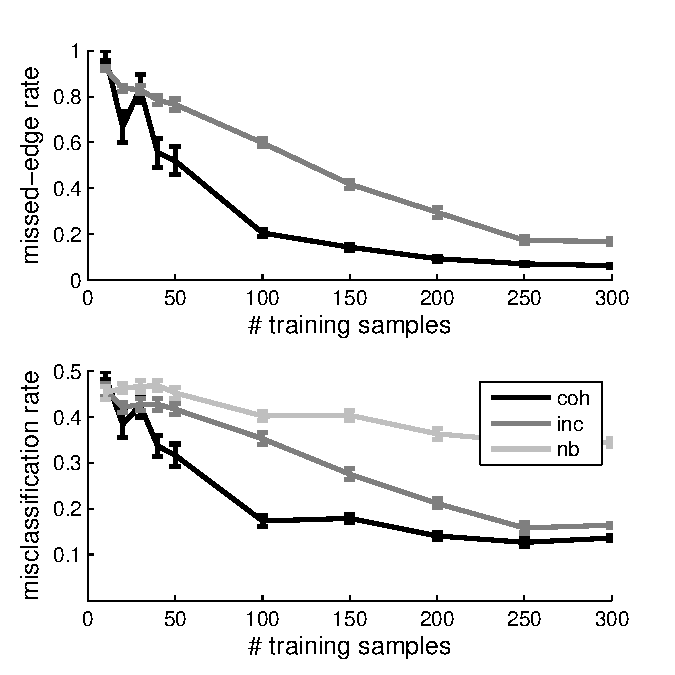
\includegraphics[width=1.0\linewidth]{../figs/homo_V70_s20_p10_q30_Lhats.pdf}
	\caption{Performance statistics as a function of sample size demonstrate that the coherent signal subgraph estimator outperforms the incoherent signal subgraph estimator, in terms of both the signal subgraph identification and classification, for the same model as in Figure \ref{fig:4x4}.  The top panel shows the missed-edge rate for each estimator as a function of the number of training samples, $n$.  The bottom panel shows the corresponding misclassification rate for the two estimators, as well as the na\"{i}ve Bayes plugin classifier.  Performance of all estimators increases monotonically with $n$ for both criteria.  Error bars show standard error of the mean here and elsewhere (averaged over 20 trials; each trial used 100 samples for held-out data). Note that $L_{chance} = 0.5 \geq \mh{L}_{NB} \geq \mh{L}_{INC} \geq \mh{L}_{COH} \geq L_* = XXX$ for essentially all $n$ here.}
	\label{fig:homo}
\end{figure}


\subsection{Relative Efficiencies} % (fold)
\label{sub:relative_efficiencies}

The above numerical results suggest that the coherent estimator outperforms the incoherent estimator.  However, that result is a function of both the model, $\mc{M}_V$ (which includes the number of vertices), and the number of samples $n$.  %Unfortunately, analytical results computing the finite sample efficiencies of each estimator are beyond our means, as is an exhaustive treatment.  Nonetheless, 
Figure \ref{fig:RE} explicitly shows that the relative performance of an estimator for a particular model changes as a function of the number of samples.  More specifically, for small $n$, the incoherent estimator yields a better performance, as indicated by by relative rate and relative efficiency being above one.  However, with more samples, when the signal subgraph is coherent, the coherent estimator will eventually outperforming the incoherent one.  At infinite samples, since both estimators are consistent, they will yield identical results: the truth.  

% we can vary $V$ and $n$, to ascertain the efficiency of the two estimators as a function of those two hyper-parameters.  Figure \ref{fig:RE} shows just such a result.  

% Given the two above estimators for the signal subgraph, a natural question is: which estimator is more efficient for a given model.  Unfortunately, the efficiency is a function of not just the model, but also the distribution and the number of samples.  Thus, we ask which estimator is more efficient for a given $\{\bth, V, n\}$ tuple.  Note that while the dependency on $V$ is redundant, in that $\bth$ is a function of $V$, we note it here to emphasize its importance in terms of relative efficiencies.  While relative efficiencies are difficult to compute analytically, below, we show a number of numerical results.


\begin{figure}[htbp]
	\centering
		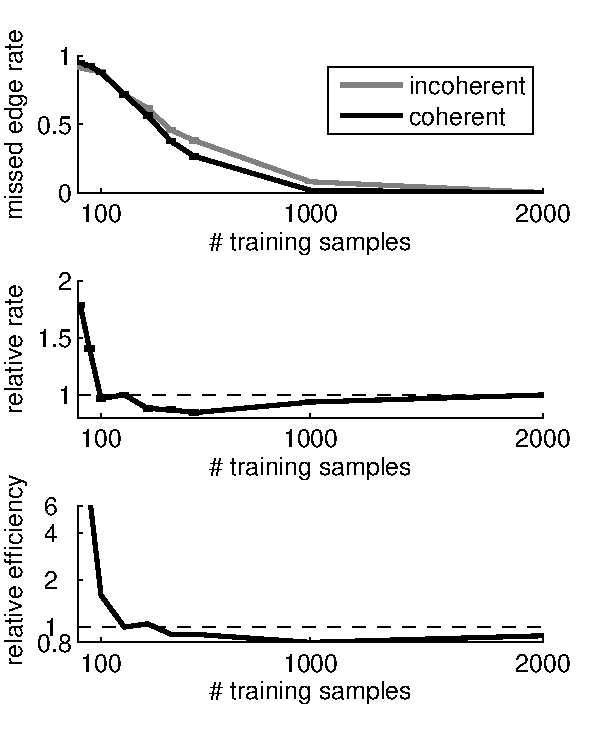
\includegraphics[width=1.0\linewidth]{../figs/RE_V30_s5_p10_q20.pdf}
	\caption{The relative performance of the coherent and incoherent estimators is a function not just of the model, but also the number of samples.  Specifically, for the model $\mc{M}_{30}(1,5;0.5,0.1,0.2)$, we compute the missed-edge rates for both the incoherent estimator (gray line) and the coherent estimator (black line).  The top panel shows that for small sample size the incoherent estimator achieves a better (lower) missed-edge rate than the coherent estimator. However, the incoherent estimator's convergence rate is slower, therefore, the coherent estimator catches up and outperforms the incoherent estimator; until both eventually converge at the truth.  The middle and bottom panels show the relative rate and efficiency curves for this model. Note that they dip below unity, and then converge back up to unity, as they must because both estimators are consistent. }
	\label{fig:RE}
\end{figure}

Thus, to choose which estimator will likely achieve best, knowledge of the model, $\mc{M}_V(m,s;\pi,p,q)$, is insufficient; rather, both the model and the number of samples must be known a priori.  

\begin{figure}[htbp]
	\centering
		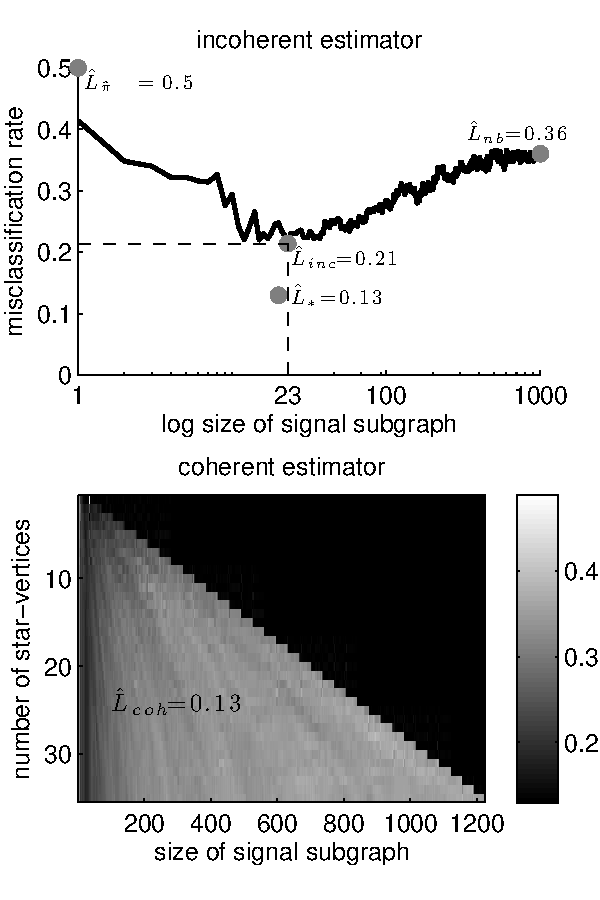
\includegraphics[width=1.0\linewidth]{../figs/coherent_image_V70_s20_p10_q30_nTr200_nTe500.pdf}
	\caption{ When constraints on the number of edges ($s$) or star-vertices ($m$) are unknown, a search over these hyperparameters can yield estimates $\mh{s}$ and $\mh{m}$.  Both panels depict held-out cross-validation error as a function of varying these parameters for the same model as in Figure 4, using 200 training samples and 500 test samples.  The left panel depicts performance of the incoherent estimator by varying the number of edges from 1 to 1000. Note that in this simulation, while $s^*=8$, $\mh{s}_{inc}=23$.  This ``conservatism'' is typical and appropriate in many model selection situations (see text for details).  The right panel shows $\mh{L}_{coh}$ as a function of both $m'$ and $s'$.  For this simulation, $\mh{m}=1$ and $\mh{s}=24$.}
	\label{fig:coherent}
\end{figure}

\begin{figure*}[htbp]
	\centering
		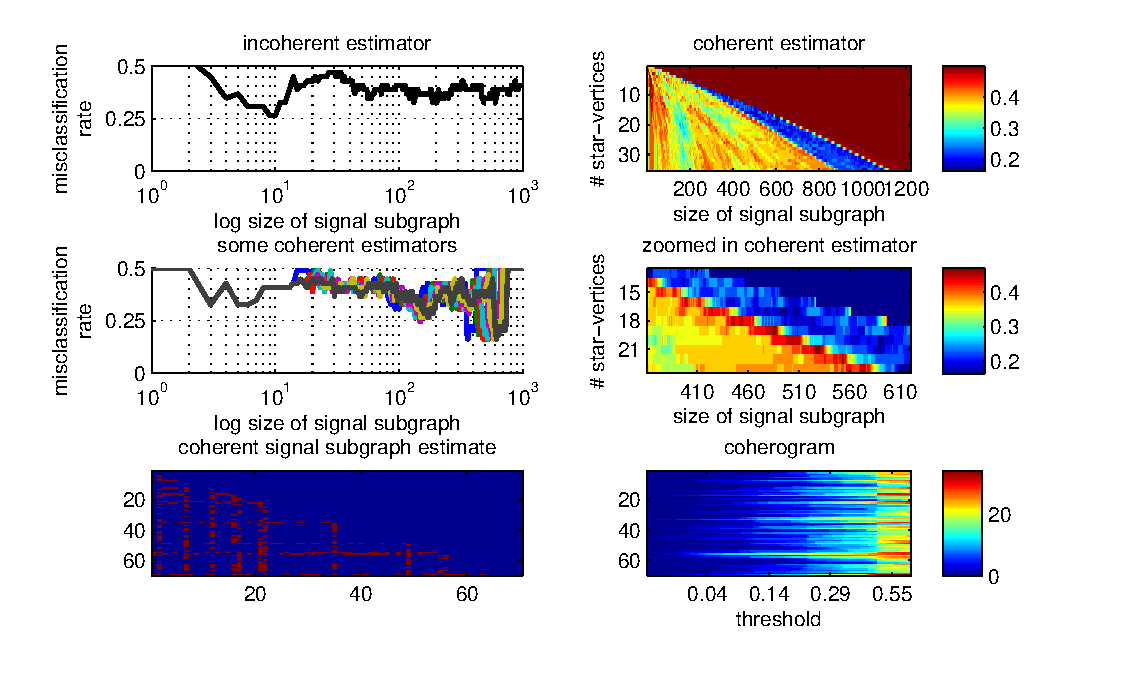
\includegraphics[width=1.0\linewidth]{../figs/BLSA0317_Count_Lhats.pdf}
	\caption{MR connectome gender signal subgraph estimation and analysis. By cross-validating over hyperparameters and models, we estimate that the ``best'' signal subgraph (for this inference task on these data) has $\mh{m}=12$ and $\mh{s}=400$.  As in the simulated data, we expect these estimates (and the particular edges in the signal subgraph) would change with more/different data. The top two panels depict the same as Figure 5.  The middle two depict misclassification rate (left) for a few different choices of $\mh{m}$ as a function of $s'$ and (right) a zoomed in depiction of the top right panel. The bottom left panel shows the estimated signal subgraph, and the bottom right shows the coherogram.  Together, these bottom panels suggest that the signal subgraph for these data is not particularly coherent.}
	\label{fig:data}
\end{figure*}


\begin{figure*}[htbp]
	\centering
		% 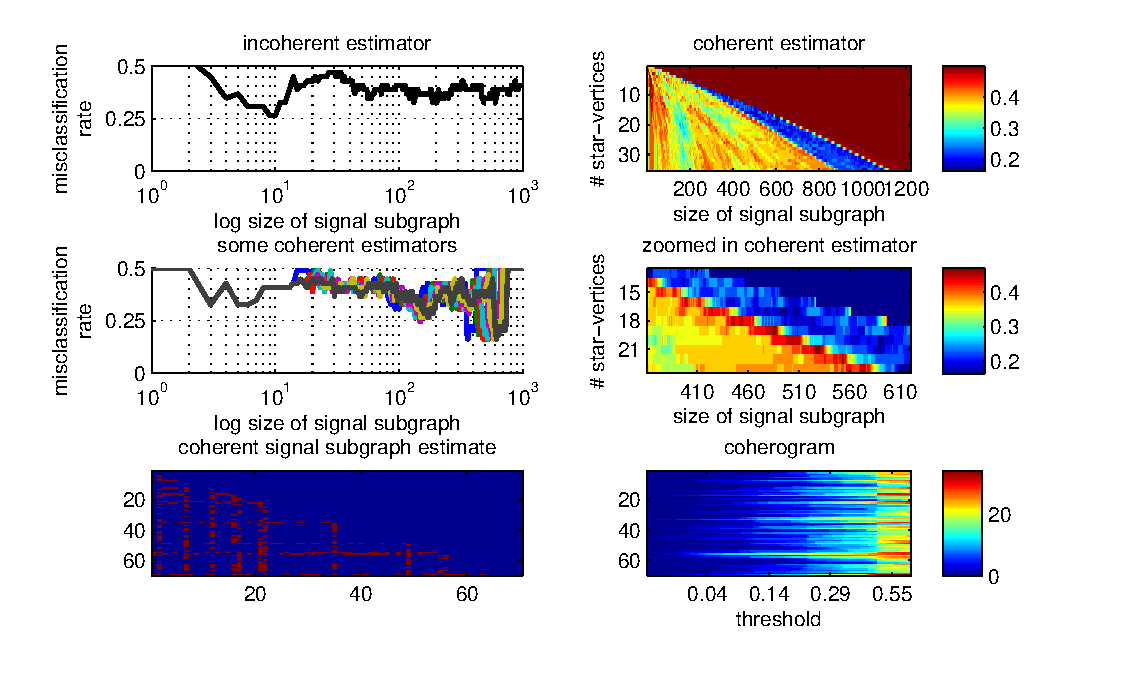
\includegraphics[width=1.0\linewidth]{../figs/BLSA0317_Count_Lhats.pdf}
	\caption{Model checking via synthetic data analysis is fundamental to understanding the performance of our estimators, and deciding how to improve them.  The top panels demonstrate that the simulated performance is better than the performance on real data, suggesting that some of the assumptions are inaccurate.  The middle panels suggest that if the model assumptions and parameter estimates were correct, than we would require approximately XXX samples before misclassification rate apparently converges (note that Bayes optimal performance is unknown in this data).}
	\label{fig:synthetic}
\end{figure*}

\clearpage
\begin{figure}[htbp]
	\centering
		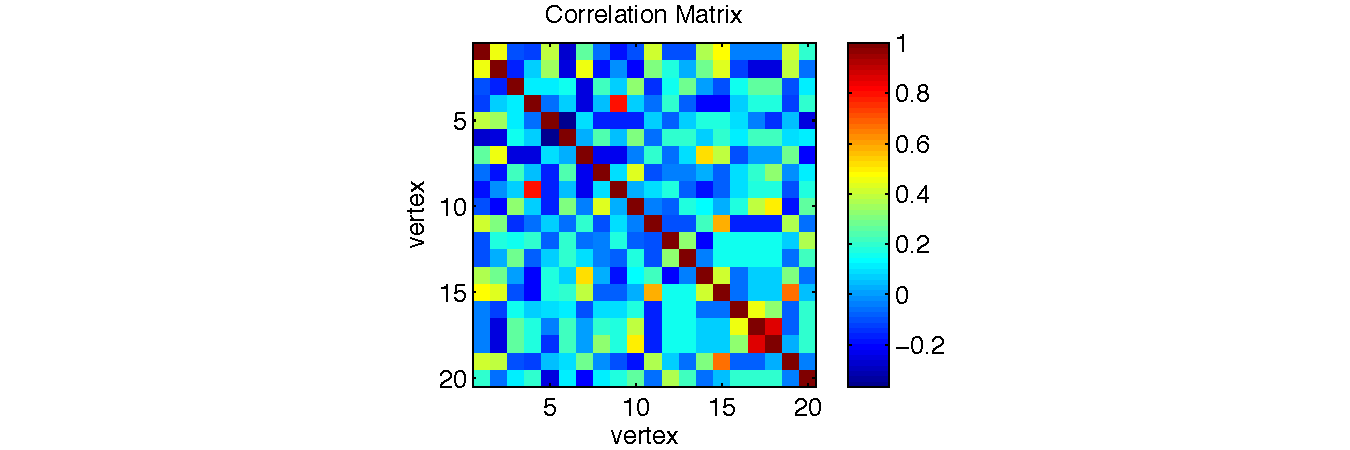
\includegraphics[width=1.0\linewidth]{../figs/cov_BLSA0317_rates_rates.pdf}
	\caption{The correlation matrix between all the edges in the coherent signal subgraph estimate. It should be clear that many of these edges, which were assumed independent, are in fact highly correlated.  This perhaps explains why the synthetic data analysis yielded improved estimates over the actual data: edges are not independent as assumed.  Moreover, this suggests that improved performance might be achieved by relaxing the independent edge assumption.}
	\label{fig:cov}
\end{figure}

% subsection subsection_name (end)


% subsection relative_efficiencies (end)

% section results (end)


\section{Discussion} % (fold)
\label{sec:discussion}

sometimes one wins B/V by doing Ess estimation:

gender data: $L_chance > L_NB > L_inc > L_coh > L_semi > L_* >= 0$


\subsection{Contributions} % (fold)
\label{sub:contributions}

$F_GY$, algs, advice, data

% subsection contributions (end)


\subsection{Next Steps} % (fold)
\label{sub:next_steps}

semi-coh, priors, proofs, relax independence (a) cond'l ind (b) m-est, model selection (short shrift), model avg (lacks interp)

% subsection next_steps (end)

\subsection{Related Work} % (fold)
\label{sub:related_work}

LASSO/ENET, low-rank+sparse, other graph classification approaches (invariants, embedding, kernels) \cite{PCP10}

% subsection related_work (end)

% section discussion (end)


% \appendices
% \section{Proof of the First Zonklar Equation}
% Appendix one text goes here.
% 
% % you can choose not to have a title for an appendix
% % if you want by leaving the argument blank
% \section{}
% Appendix two text goes here.

% use section* for acknowledgement
\ifCLASSOPTIONcompsoc
  % The Computer Society usually uses the plural form
  \section*{Acknowledgments}
\else
  % regular IEEE prefers the singular form
  \section*{Acknowledgment}
\fi


% Can use something like this to put references on a page
% by themselves when using endfloat and the captionsoff option.
\ifCLASSOPTIONcaptionsoff
  \newpage
\fi


\bibliography{/Users/jovo/Research/latex/library}
\bibliographystyle{IEEEtran}

\begin{IEEEbiography}{Joshua T. Vogelstein}
Biography text here.
\end{IEEEbiography}

% if you will not have a photo at all:
\begin{IEEEbiographynophoto}{John Doe}
Biography text here.
\end{IEEEbiographynophoto}

% insert where needed to balance the two columns on the last page with
% biographies
%\newpage

\begin{IEEEbiographynophoto}{Jane Doe}
Biography text here.
\end{IEEEbiographynophoto}

% Can be used to pull up biographies so that the bottom of the last one
% is flush with the other column.
%\enlargethispage{-5in}

\end{document}



